\section{Graphics Processing Units}
Dedicated Graphic Processsing Units (``GPUs'') are very common in desktop and laptops. \citep{STEAMHW}
GPUs are commonly used in the private and professional world, for computer gaming and accelerating graphic intensive programs such as Adobe Photoshop and 3D modeling tools. \citep{NVIDIAADOBE}
Their architecture can also be used for certain types of computations, primarily computations which can be done in parallel. 

\begin{figure}[h!]
\centering
 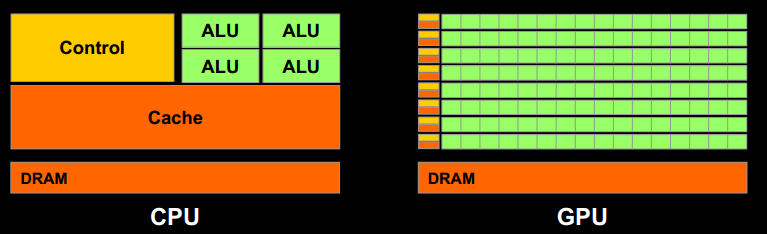
\includegraphics[width=1\textwidth]{figures/GPUCPUimage.png} % trim=4.85cm 15cm 0.85cm 1cm
\caption{A basic representation of the Transistor allocation on a GPU compared to a CPU}\label{image:GPUCPUimage} %ftp://download.nvidia.com/developer/cuda/seminar/TDCI_Arch.pdf
\vspace{-15pt}
\end{figure}

A basic layout comparsion of a Centeral Processing Unit (``CPU'') and a GPU is shown in \myref{image:GPUCPUimage}.
In the GPU there are many less powerfull cores, however the total computation capacity is higher. 
As of Q1 2015 an example of a modern high end desktop CPU is the Intel Haswell core i7 5960X which has a theoretical peak of 384 giga- floating operations pr. secound (GFLOPS) over 8 cores. \citep{puget}
A contemporary high end GPU is the NVIDIA GTX 980 which has 4616 GFLOPS, for single precision with 2048 Shading Units. \citep{techpowerup}
This results in the GPU having 12 times more FLOPS, meaning that it can process more data. 

This makes GPU an obvious target for computation, even some which are not graphical. % Antagende/konkluderende?!?